\scanpage{57}
\mspage{\handwritten{24.}}
% archive sheet number: 56

il s'agit donc de montrer que $K$ est affine.

\deleted{Le théorème est connu dans le cas où $k$ est algébriquement clos\unsure{,} et où $G$ et $H$ sont réduits (Chevalley}\inserted{\deleted{\handwritten{Supposons d'abord.}}}
\margin{\handwritten{\makebox[0pt][l]{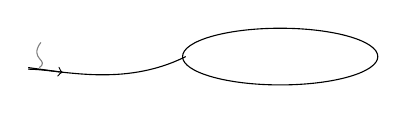
\begin{tikzpicture}[x=.4cm,y=.4cm,baseline=0pt]\draw (3.1,0) ellipse (3.1 and .9);\draw (.1,0).. controls (-1.9,-1) and (-3.9,-.4)..(-4.9,-.4);\draw[->] (-4.9,-.35)--(-3.8,-.5);\draw[gray,thin] (-4.5,.45).. controls (-4.9,-.1) and (-4.2,-.1)..(-4.55,-.35);\end{tikzpicture}}VOIR CI CONTRE}}

Dans le cas où $k$ est algébriquement clos, et $G$ et $H$ quelconques,\deleted{(\unsure{$(G/H)_{\mathrm{red}}$|?} est \unsure{isomorphe|?} à \unsure{$G_{\mathrm{red}}/H_{\mathrm{red}}$} réduit (\unsure{9.2 vi|9.2 iv|2.2 ?})}, $(G\handwritten{\times}_k H)_{\mathrm{red}}$ est isomorphe à $(G_{\mathrm{red}})\handwritten{\times}_k(H_{\mathrm{red}})$, donc $(G_{\mathrm{red}})/(H_{\mathrm{red}})$ est isomorphe à $(G/H)_{\mathrm{red}}$. Puisque $(G_{\mathrm{red}})/H_{\mathrm{red}}$ est affine, il en est de même de $G/H$ (EGA I 5.1.10), car, puisque $G/H$ est de type fini sur $k$, son nilradical est nilpotent.

Dans le cas où $k$ est quelconque, $G\handwritten{\otimes}_k\handwritten{\bar{k}}/H\handwritten{\unsure{\oslash|\otimes}}_k\handwritten{\bar{k}}$ est isomorphe à $(G/H)\handwritten{\otimes}_k\handwritten{\bar{k}}$ (9.2 v)), donc puisque le premier est affine, il en est de même du second, donc $G/H$ est affine\handwritten{(ref.)\unsure{'|,}}
\margin{\handwritten{(\qquad)}}

\uline{Deuxième cas} : \deleted{c}\handwritten{C}as général . D'après (11.13), l'algèbre $A$ de $G$ est limite inductive d'une famille filtrante croissante $(A_i)_{i\in I}$ de sous-algèbres de type fini de $A$ stables par l'application diagonale et l'involution. D'après (\deleted{Exp.}\inserted{EGA} I 4.2.3), $H$ est affine, et si on note $B$ l'algèbre de $H$, l'homomorphisme $A\handwritten{\longrightarrow}B$ déduit de l'injection $H\handwritten{\longrightarrow}G$ est surjectif. Posons $I=\operatorname{Ker}(A\handwritten{\to}B)$, $I_i=I\handwritten{\cap}A_i$ et $B_i=A_i/I_i$; puisque la structure d'hyperalgèbre associative augmentée involutive de $A$ passe au quotient à travers $I$, on vérifie aisément que celle de $A_i$ passe au quotient à travers $I_i$, si bien que $B_i$ est l'algèbre d'un $k$-groupe affine de type fini $H_i$; il est clair que $B=\lim B_i$. D'après (EGA I 4.2.3), $H_i$ est isomorphe à un sous-préschéma en g\inserted{\handwritten{r\begin{tikzpicture}[x=1cm,y=1cm,baseline=-.1cm]\draw[thin] (-.25,.05)--(-.18,-.3).. controls (-.03,-.12) and (.17,-.17)..(.25,-.1);\end{tikzpicture}}}oupes fermé de $G_i$. D'après (6.7) le fait que $H$ soit invariant dans $G$ s'exprime en disant qu'un certain morphisme $H\handwritten{\times}_k G\handwritten{\longrightarrow}G$ se factorise à travers l'injection $H\handwritten{\longrightarrow}G$, autrement dit que l'homomorphisme correspondant $A\handwritten{\longrightarrow}B\handwritten{\otimes}_k A$ se factorise à travers l'homomorphisme canonique $A\handwritten{\longrightarrow}B$; on vérifie aisément que l'homomorphisme $A_i\handwritten{\longrightarrow}B_i\handwritten{\otimes}_k A_i$ défini de manière analogue se factorise à travers $A_i\handwritten{\longrightarrow}B_i$, donc que $H_i$ est invariant dans $G_i$. D'après ce qui a été vu précédemment, $G_i$ étant de type fini sur\inserted{\handwritten{\ \begin{tikzpicture}[x=1cm,y=1cm,baseline=0cm]\draw[thin] (0,.3)--(-.03,-.35);\end{tikzpicture}}}$k$, $G_i/H_i$ est représentable par un $k$-groupe affine $K_i$, dont nous noterons $C_i$ l'algèbre. Posons alo\makebox[0pt][l]{\raisebox{.8ex}{\handwritten{\unsure{4|\deleted{4}|r|?}}}}rs $C=\underset{\handwritten{\longrightarrow}}{\lim}C_i$, et soit $K=\underset{\handwritten{\longleftarrow}}{\lim}K_i$ le $k$-préschéma affine d'algèbre $K$ (EGA IV 8.2.3).

\margin{\figure{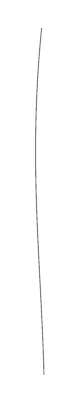
\begin{tikzpicture}[x=1cm,y=1cm]\draw[gray,thin] (0,0).. controls (-.04,1.5) and (-.2,2.7)..(-.03,4.4);\end{tikzpicture}}}

Montrons que $K$ représente $G/H$; pour cela, il suffit de vérifier que \deleted{le diagramme}
\margin{\handwritten{est ce défini ?}}
\diagram{\begin{tikzcd}[ampersand replacement=\&,execute at end picture={\draw[gray,thin] ([xshift=1cm]current bounding box.center) ellipse [x radius=4.2cm,y radius=.55cm];}]
H\handwritten{\times}_k G \arrow[r,"\handwritten{\unsure{\sim|\longrightarrow}}"] \& G \arrow[r,"{\handwritten{\times_K}}" description,pos=.25] \& \deleted{\unsure{K|H}}\handwritten{G}
\end{tikzcd}\quad\deleted{est cartésien}}
\handwritten{,} et que le morphisme $G\handwritten{\longrightarrow}K$ est couvrant pour la topologie fpqc. (\deleted{\unsure{Exp.}} IV 4.4.3). Or, \deleted{chacun des diagrammes}\inserted{\handwritten{pour chaque $i$, on \unsure{a|-}}}
\diagram{\begin{tikzcd}[ampersand replacement=\&]
H_i\handwritten{\times}_k G_i \arrow[r,"\handwritten{\unsure{\sim|\longrightarrow}}"] \& G_i \arrow[r,"{\handwritten{\times_{K_i}}}" description,pos=.25] \& \deleted{\unsure{K|H}}\handwritten{G}_i
\end{tikzcd}}
\handwritten{,}\deleted{étant cartésien,}\inserted{\handwritten{donc}} il en est de même d\deleted{\unsure{e|u}}\handwritten{u} \deleted{diagramme}\inserted{\handwritten{morphisme\begin{tikzpicture}[x=1cm,y=1cm,baseline=-.1cm]\draw[thin] (0,.06).. controls (.18,-.15) and (-.85,-.1)..(-.9,-.3)--(-.85,-.47);\end{tikzpicture}}} obtenu en passant à la limite projective; enfin chacun des morphismes
